% !TeX spellcheck = en_US

%--------------------------Set the variables for every client---------------------
\renewcommand{\hostname}{machineA}
\renewcommand{\os}{\textit{Ubuntu 16.04 LTS}}
\renewcommand{\ip}{XX.XX.XX.XX}

\renewcommand{\vuln}{}
\renewcommand{\product}{}
%The x-Variables are only used, when root is defined (== root shell)
\renewcommand{\vulnx}{\vulnPassword}
\renewcommand{\productx}{}
%%%Did you get root? Comment out if you only got low priv access 
\def\gotroot{}   %%% Define root if you got root shell
%\undef\gotroot % Else undefine

%-------------------------------Auto generated content-----------------------------%----------------------------------------------------------------------------------
\subsection{\label{\hostname}\hostname}

\textit{Note: This machine is fictional and unrelated to Offensive Security machines. Details have been fabricated for purposes of example.}

\subsubsection{Service Enumeration}

\ip\ was scanned with the following switches and relevant output:
\par \texttt{nmap -iL targets -A -oA basicscan}

\begin{lstlisting}[caption={Nmap scan},label={lst:nmap}]
	...
	Nmap scan report for XX.XX.XX.XX
	Host is up (0.12s latency).
	Not shown: 998 closed ports
	PORT   STATE SERVICE VERSION
	...
	80/tcp open  http    Apache httpd 2.4 ((Ubuntu))
	...
\end{lstlisting}



%-------------------------------REMOTE ACCESS---------------------------------

\subsubsection{Remote Access Exploitation}

\paragraph{Vulnerability Discussion} 
% Using \vulnPassword defined in maindocument.tex
\vulnPassword: Malicious users can upload a reverse shell through the backend management interface by exploiting weak administrative credentials.

\paragraph{Recommendations}
Inform users about the importance of strong authentication to security efforts\footnote{Official Microsoft password guidance: \url{https://www.microsoft.com/en-us/research/wp-content/uploads/2016/06/Microsoft_Password_Guidance-1.pdf}}. Additionally, disable remote web access to the management interface.


\paragraph{Proof of Concept}

\osid\ searched for attack vectors in \fullhostname's web services by using Gobuster to brute force files and directories on \url{http://XX.XX.XX.XX}.\\
\texttt{gobuster dir -w /var/lists/dirbuster_medium --url http://XX.XX.XX.XX}
\begin{lstlisting}[caption={Gobuster output.}, label={lst:gobuster}]
	===============================================================
	Gobuster v3.0.1
	by OJ Reeves (@TheColonial) & Christian Mehlmauer (@_FireFart_)
	===============================================================
	[+] Url:            http://XX.XX.XX.XX
	[+] Threads:        20
	[+] Wordlist:       /var/lists/dirbuster_medium
	[+] Status codes:   200,204,301,302,307,401,403
	[+] User Agent:     gobuster/3.0.1
	[+] Extensions:     php
	[+] Timeout:        10s
	===============================================================
	2020/04/20 00:04:20 Starting gobuster
	===============================================================
	/index.php (Status: 200)
	/example_backdoor.php (Status: 200)
	===============================================================
	2020/04/20 00:04:20 Finished
	===============================================================	
\end{lstlisting}

Browsing to \url{http://XX.XX.XX.XX//example_backdoor.php} retrieved a management interface. 
\texttt{} 

\begin{figure}[H]
	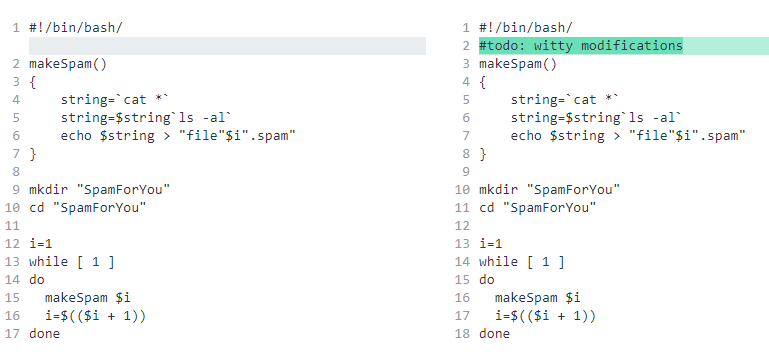
\includegraphics [width=.75\textwidth]{./hosts/\hostname/image1.png}
	\caption{Management interface. \\ Note: Image sourced from \nolinkurl{http://www.apachegui.net/images/Control.png}.}
	\label{fig:obviouscreds}
\end{figure}

The management interface authentication used weak credentials. \osid\ logged in with username \texttt{Admin} and password \texttt{Password}.

\osid\ then did stuff to gain a low-privilege remote shell.

After doing stuff, \osid\ exfiltrated evidence of the low-privilege shell.

\begin{figure}[H]
	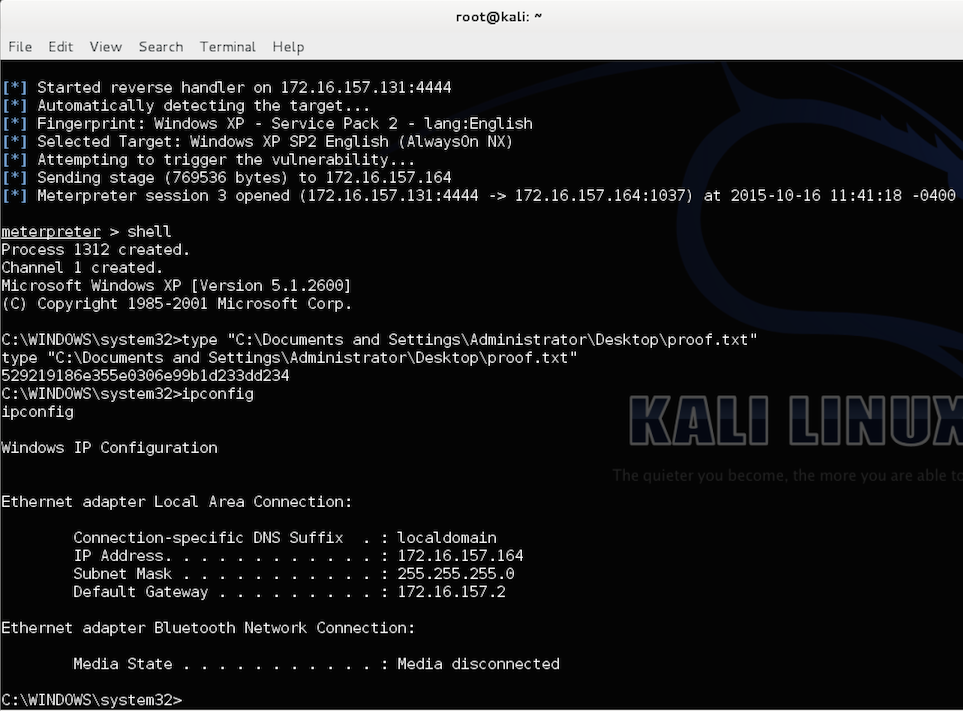
\includegraphics [width=.75\textwidth]{./hosts/\hostname/image2.png}
	\caption{Proof of succesful low-privilege remote access to \fullhostname. \\
		Note: Image sourced from \url{https://support.offensive-security.com/oscp-exam-guide/}. Ensure \texttt{type} or \texttt{cat} are used to print the flag and \texttt{ipconfig} or its counterparts to display the machine's address.}
\end{figure}

%-------------------------------PRIVILEGE ESCALATION---------------------------------
\ifdefined\gotroot
\subsubsection{Privilege Escalation}
\paragraph{Vulnerability Discussion}
\vulnCow\ allows privilege escalation of a low-privilege shell. \osid\ exploited the vulnerability to gain root access on \hostname.
\paragraph{Recommendations}
The vendors of \os\ are aware of the privilege escalation vulnerability\footnote{Official support article: \url{https://ubuntu.com/blog/dirty-cow-was-livepatched-in-ubuntu-within-hours-of-publication}}. Follow vendor instructions to remediate vulnerability.

\paragraph{Proof of Concept}

\osid\ exploited \vulnCow. See \ref{sec:vulnCowDiff} for exploit modification details.

\osid\ was then able to exfiltrate the \nolinkurl{proof.txt} key and network configuration.

\begin{figure}[H]
	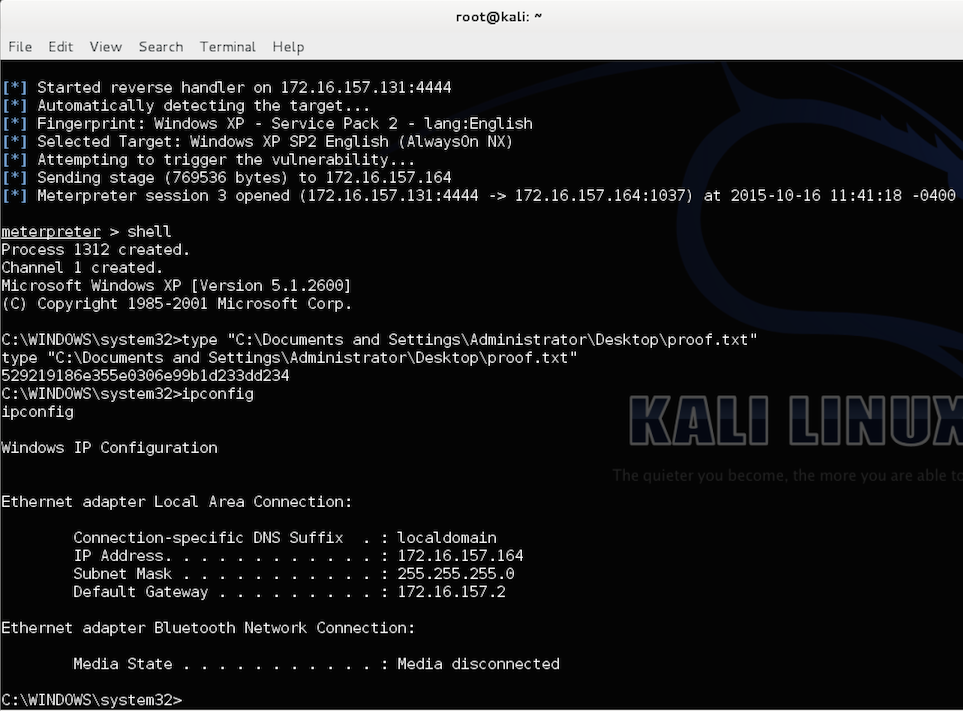
\includegraphics [width=.75\textwidth]{./hosts/\hostname/image2.png}
	\caption{Proof of successful \textit{root} access to \fullhostname. \\Note: Image sourced from \url{https://support.offensive-security.com/oscp-exam-guide/}. Ensure \texttt{type} or \texttt{cat} are used to print the flag and \texttt{ipconfig} or its counterparts to display the machine's address.}
\end{figure}
\fi